\documentclass[sigconf]{acmart}
\pagestyle{fancy}
\settopmatter{printacmref=false}
\renewcommand\footnotetextcopyrightpermission[1]{}
\pagestyle{plain}
\fancyhead{}
\settopmatter{printacmref=false, printfolios=false}
\setcopyright{none}
\settopmatter{printacmref=false}
\acmDOI{}


\setlength{\parskip}{0pt}
\setlength{\parsep}{0pt}
\setlength{\headsep}{0pt}
\setlength{\topskip}{0pt}
\setlength{\topmargin}{0pt}
\setlength{\topsep}{0pt}
\setlength{\partopsep}{0pt}
\setlength{\textfloatsep}{8pt plus 2pt minus 2pt}
\emergencystretch=1em
\usepackage{mdwlist}
\usepackage{amsmath}
\usepackage{graphicx}
\usepackage{booktabs}
\usepackage{array}
\usepackage{pgfplots}
\pgfplotsset{compat=1.17}
\definecolor{chartblue}{HTML}{2A78D6}
\definecolor{chartorange}{HTML}{EB6834}


\begin{document}
\title{\mbox{\scalebox{0.985}[1]{Evaluating Ocean Drift Prediction from Wind and Location Data}}}
\titlenote{Code and data: \url{https://github.com/jakecush1/autonomous-pilot-ML}}
\author{Jake Cushway}
\affiliation{
  \institution{University of Victoria}
  \city{Victoria}
  \country{Canada}
}
\email{jakecush1@uvic.ca }

\author{Rowan Hall}
\affiliation{
  \institution{University of Victoria}
  \city{Victoria}
  \country{Canada}
}
\email{rowanhall@uvic.ca }


\begin{abstract}
DataXplorer is an uncrewed surface vehicle (USV) that serves as a weather station off Half Moon Bay, California, and must stay within 10~nautical miles (NM) of the retired NOAA buoy 46012. We forecast its position one hour ahead from onboard wind and GPS data alone, comparing an LSTM and a Transformer with persistence and linear regression on 94~days of 1-minute telemetry. On unseen November data both beat the baselines: the LSTM's median error is 213~m, 30\% below persistence. Code and data: \mbox{\url{https://github.com/jakecush1/autonomous-pilot-ML}}.
\end{abstract}

\keywords{Uncrewed surface vehicle, drift prediction, LSTM, transformer}
\maketitle
\pagestyle{empty}
\brokenpenalty=100

\section{Introduction}
Pilots keep DataXplorer on station by watching its position and repositioning it; a reliable drift forecast would let them intervene only when needed. Operational drift models such as GNOME~\cite{zelenke2012gnome} and leeway models~\cite{breivik2011leeway} move an object with a fitted fraction of the wind on top of forecast currents. We instead learn the drift from the USV's own record, and test whether an LSTM~\cite{hochreiter1997lstm} and a Transformer~\cite{vaswani2017attention} improve on persistence and linear regression.


\section{Research Questions}
\noindent\textbf{RQ1.} Do the sequence models predict the USV's position one hour ahead more accurately than the baselines, and which model is best? Answering this shows whether learning patterns within the past hour, such as the drift turning or slowing, is worth the extra complexity. In response, we benchmark both against persistence and linear regression by their endpoint error on the final test set.


\noindent\textbf{RQ2.} How much does wind contribute to predicting drift? We expected wind to be the main driver of drift, since it both pushes on the USV and drives the surface current.
Leeway models treat it as such~\cite{breivik2011leeway}, and it is one of only two inputs our models use. In response, we measure how often the USV drifts with the wind, how much of the drift a linear fit on the wind explains, and how the linear regression's error changes without its wind features.


\noindent\textbf{RQ3.} How sensitive are the LSTM and the Transformer to their learning rate? Both were trained with an untuned learning rate, so this checks whether their performance depends on that choice. In response, we retrain each model with four learning rates and compare the validation errors.


\begin{table}[t]
\centering\footnotesize
\caption{Dataset statistics over all nine deployments.}
\label{tab:dataset}
\begin{tabular}{@{}ll@{}}
\toprule
Deployments            & 9 (Apr 17 -- Nov 16, 2026) \\
Records (1 per minute) & 135{,}234 (93.9 days) \\
Missing values         & 11.0\% of records \\
Motor off              & 50.3\% of minutes \\
Valid drift minutes    & 66{,}803 (46.4 days) \\
Samples (dev.\ / final test) & 30{,}303 / 3{,}920 \\
Drift speed (median)   & 0.44\,kn \\
Wind speed (mean / max)& 10.0 / 28.2\,kn \\
Wind direction         & 54\% from the NW \\
\bottomrule
\end{tabular}
\end{table}

\section{Dataset}
The data was collected directly from DataXplorer by Open Ocean Robotics at the site of NOAA buoy 46012; we exported only the channels this experiment needs (time, GPS position, wind speed and direction, and motor power), and the files are in our repository. They cover nine deployments from April to November 2026 (Table~\ref{tab:dataset}). A minute is valid when the motor is off, the vessel moves slower than 3~kn (faster means a tow) and no value is missing after gaps of up to 5~minutes are interpolated. A sample needs 120 consecutive valid minutes: the past hour is the input, with four features per minute (movement and wind push, each east and north), and the movement over the next hour, read from later GPS positions, is the target. This gives 34{,}223 samples. No public benchmark covers this vessel, so its own record at the site of use is the most relevant data; it covers one vessel, with no winter or current data.


\section{Baselines}

We compare the LSTM and Transformer with two baselines. All four models use the same samples, cleaning and metric.

\textbf{Persistence} predicts that the next hour's movement repeats the last hour's. It needs no training, has no hyperparameters, and is the bar every model must beat.

\textbf{Linear regression} predicts the next hour's movement from six numbers summarizing the past hour: the movement, the current wind and the mean wind, each east and north. Like a leeway model~\cite{breivik2011leeway}, it moves the USV linearly with the wind, on top of a term for its past drift, so it tests whether a linear model suffices before turning to nonlinear ones. We use \texttt{LinearRegression} from scikit-learn, which has no hyperparameters to tune.


\textbf{LSTM and Transformer.} Unlike the two baselines, the LSTM and the Transformer read the past hour as 60 one-minute steps of movement and wind. The LSTM~\cite{hochreiter1997lstm} processes the minutes in order, updating its memory at each step. The Transformer~\cite{vaswani2017attention} instead looks at all 60 minutes at once, using attention to weigh each minute against every other. Both have two layers of width 64, predict the movement east and north over the next hour, and are implemented in PyTorch and trained with Adam~\cite{kingma2015adam}.


\begin{figure}[t]
\centering
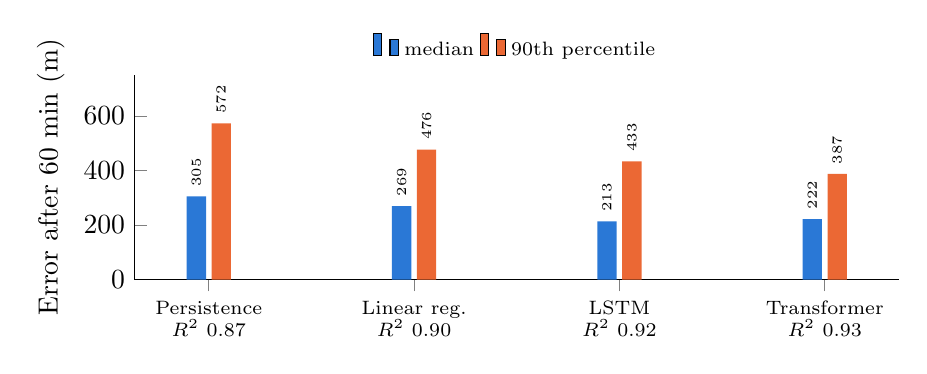
\begin{tikzpicture}
\begin{axis}[
    ybar, bar width=7pt,
    scale only axis, width=0.8\columnwidth, height=2.6cm,
    ymin=0, ymax=750, ytick={0,200,400,600},
    ylabel={Error after 60 min (m)},
    xtick={1,2,3,4},
    xticklabels={{Persistence\\$R^2$ 0.87}, {Linear reg.\\$R^2$ 0.90}, {LSTM\\$R^2$ 0.92}, {Transformer\\$R^2$ 0.93}},
    xticklabel style={align=center, font=\scriptsize},
    enlarge x limits=0.12,
    axis lines*=left,
    nodes near coords,
    nodes near coords style={font=\tiny, rotate=90, anchor=west},
    legend style={at={(0.5,1.02)}, anchor=south, legend columns=2, font=\scriptsize, draw=none},
]
\addplot[fill=chartblue, draw=none] coordinates {(1,305) (2,269) (3,213) (4,222)};
\addplot[fill=chartorange, draw=none] coordinates {(1,572) (2,476) (3,433) (4,387)};
\legend{median, 90th percentile}
\end{axis}
\end{tikzpicture}
\Description{Vertical bar chart of the median and 90th-percentile endpoint error on the final test set:
persistence 305 and 572 m (R-squared 0.87), linear regression
269 and 476 m (0.90), LSTM 213 and 433 m (0.92), Transformer 222 and 387 m (0.93).}
\caption{Endpoint error on the final test set (November).}
\label{fig:results}
\end{figure}


\section{Evaluation Strategy and Metrics}

\textbf{Splits.} Neighbouring samples overlap almost completely, so instead of a random split we split by deployment in time order: April--October form the development set (30{,}303 samples, 89\%) and November the final test set (3{,}920 samples), scored once after all settings were fixed. Within the development set, the latest deployment (October 16--23) is the validation set, in place of $n$-fold cross-validation, so that training (April to October~13) always precedes validation in time; it is used for early stopping and for RQ3.

\textbf{Metric.} The endpoint error is the distance in metres between the predicted and the true position after 60 minutes. We report its median (a typical miss) and 90th percentile (a bad case, usable as a safety radius), and $R^2$, the share of the variation in the movement that a model explains; classification metrics do not apply.

\textbf{Hyperparameters.}
Both networks are trained on the mean squared error with a learning rate of $10^{-3}$ and batches of 256 samples; inputs and targets are standardized using training statistics only. Training runs for up to 80 epochs, stops after 10 epochs without improvement, and keeps the epoch with the lowest validation error. These settings were not tuned before the final test; RQ3 varies the learning rate (Table~\ref{tab:rq3}). All runs use seed~0.


\section{Results and Discussion}


\textbf{RQ1: do the sequence models beat the baselines?} Figure~\ref{fig:results} shows that both sequence models outperform both baselines on the final test set. The LSTM has the lowest median error, 213~m, 30\% below persistence and 21\% below linear regression, while the Transformer has the lowest 90th percentile, 387~m, 32\% below persistence; both explain 92--93\% of the variation ($R^2$). This can be attributed to the sequence models reading the past hour minute by minute, so they see the drift turn or slow, whereas persistence assumes the last hour repeats and linear regression sees only its totals. Persistence still more than halves the error of assuming no drift (747~m), because the current changes slowly (RQ2), and linear regression beats it only through its wind features. With one seed per model, the 9~m gap between the two may be noise.


\textbf{RQ2: how much does wind contribute?} Figure~\ref{fig:withwind} shows that wind steers the drift but does not dominate it. On the development set, the USV drifts within $\pm45^\circ$ of downwind 47\% of the time, against 25\% if wind had no effect; the share rises from 20\% below 5~kn, no better than chance, to 87\% above 15~kn. This can be attributed to the balance between wind and current: in light wind the current sets the direction, and only a strong wind overcomes it. The drift along the wind grows by 4.2\% of the wind speed, near the 1--4\% windage GNOME assumes~\cite{zelenke2012gnome}, yet the wind vector explains only about a quarter of the drift ($R^2 = 0.23$). The value of wind for prediction therefore depends on the weather: removing the wind features from the linear regression raises its median error on the final test set from 269 to 301~m, but by only 2~m on the validation week, which was much calmer (an hourly mean wind of at least 10~kn in 34\% of samples, against 73\% in November).

\begin{figure}[t]
\centering
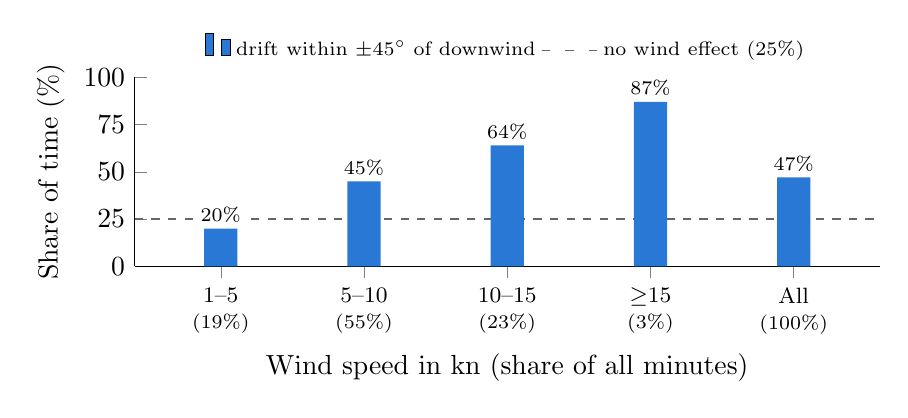
\begin{tikzpicture}
\begin{axis}[
    ybar, bar width=12pt,
    scale only axis, width=0.78\columnwidth, height=2.4cm,
    ymin=0, ymax=100, ytick={0,25,50,75,100},
    ylabel={Share of time (\%)},
    xlabel={Wind speed in kn (share of all minutes)},
    xtick={1,2,3,4,5},
    xticklabels={{1--5\\\scriptsize(19\%)}, {5--10\\\scriptsize(55\%)},
                 {10--15\\\scriptsize(23\%)}, {$\geq$15\\\scriptsize(3\%)}, {All\\\scriptsize(100\%)}},
    xticklabel style={align=center, font=\footnotesize},
    enlarge x limits=0.15,
    axis lines*=left,
    nodes near coords={\pgfmathprintnumber{\pgfplotspointmeta}\%},
    nodes near coords style={font=\scriptsize, fill=white, inner sep=1pt, yshift=1pt},
    legend style={at={(0.5,1.03)}, anchor=south, legend columns=2, font=\scriptsize, draw=none},
]
\draw[dashed, black!60] (rel axis cs:0,0.25) -- (rel axis cs:1,0.25);
\addplot[fill=chartblue, draw=none] coordinates {(1,20) (2,45) (3,64) (4,87) (5,47)};
\addlegendentry{drift within $\pm45^\circ$ of downwind}
\addlegendimage{line legend, dashed, black!60}
\addlegendentry{no wind effect (25\%)}
\end{axis}
\end{tikzpicture}
\Description{Bar chart of the share of time the USV drifts within 45 degrees of downwind:
20\% at 1--5 kn, 45\% at 5--10 kn, 64\% at 10--15 kn, 87\% above 15 kn and 47\% overall,
against 25\% expected if wind had no effect on direction.}
\caption{Share of time drifting downwind, by wind speed.}
\label{fig:withwind}
\end{figure}

\textbf{RQ3: how sensitive are the models to their learning rate?} Table~\ref{tab:rq3} shows that both models are moderately sensitive, in opposite directions. The LSTM's median validation error falls steadily from 257~m to 223~m as the rate grows; its best rate, $3{\times}10^{-3}$, is 13~m (median) and 50~m (90th percentile) better than the default of $10^{-3}$, so its optimum may lie above the range we tested. The Transformer stays within 241--252~m up to the default, its best setting, but worsens to 267~m at $3{\times}10^{-3}$. Both stay below persistence (294~m) at every setting, so the advantage found in RQ1 holds across the whole range. This can be attributed to early stopping, which absorbs a slower start: a smaller rate only delays the best epoch (epoch 8--11 at $10^{-4}$, against 1--2 at the default). The largest rate is too large for the Transformer, which is usually trained with a warm-up~\cite{vaswani2017attention}.

\begin{table}[!ht]
\centering\footnotesize
\caption{Validation error by learning rate: median / 90th (m).}
\label{tab:rq3}
\begin{tabular}{@{}lcccc@{}}
\toprule
Learning rate & $10^{-4}$ & $3{\times}10^{-4}$ & $10^{-3}$ & $3{\times}10^{-3}$ \\
\midrule
LSTM        & 257 / 531 & 249 / 529 & 236 / 541 & 223 / 491 \\
Transformer & 249 / 516 & 252 / 513 & 241 / 513 & 267 / 529 \\
\bottomrule
\end{tabular}
\end{table}


\textbf{Reproducibility.} With fixed seeds, \texttt{bash quickstart.sh} installs the pinned dependencies and reruns every step behind Table~\ref{tab:dataset}, RQ1 and RQ2, from the raw telemetry to the scores in \path{evaluation/results/}, in about 5~minutes on a laptop CPU. For RQ3, set \texttt{LR} in \path{src/models/nn_models.py} and rerun the \texttt{lstm} and \texttt{transformer} steps.


\bibliographystyle{ACM-Reference-Format}
\bibliography{bibliography.bib}

\end{document}
